\section{Example Run with Released  Application}\label{sec:app}

%###################################
%###################################
%###################################
\begin{figure}[!ht]
\centering
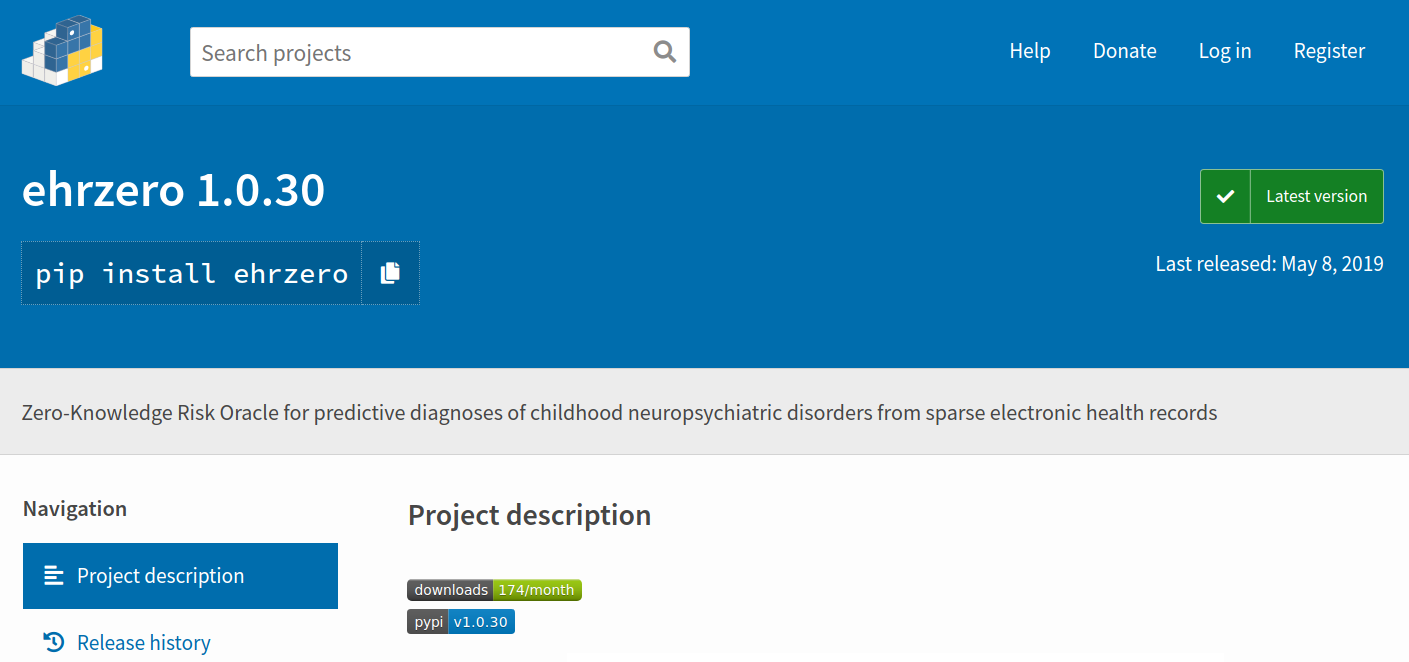
\includegraphics[width=.9\textwidth]{Figures/scrn}
\captionN{Screen capture of the page on pypi.org hosting the released application Link: \href{hhtp://pypi.org/ehrzero}{http://pypi.org/ehrzero}}
\end{figure}
%###################################

\begin{figure}[!ht]
\centering
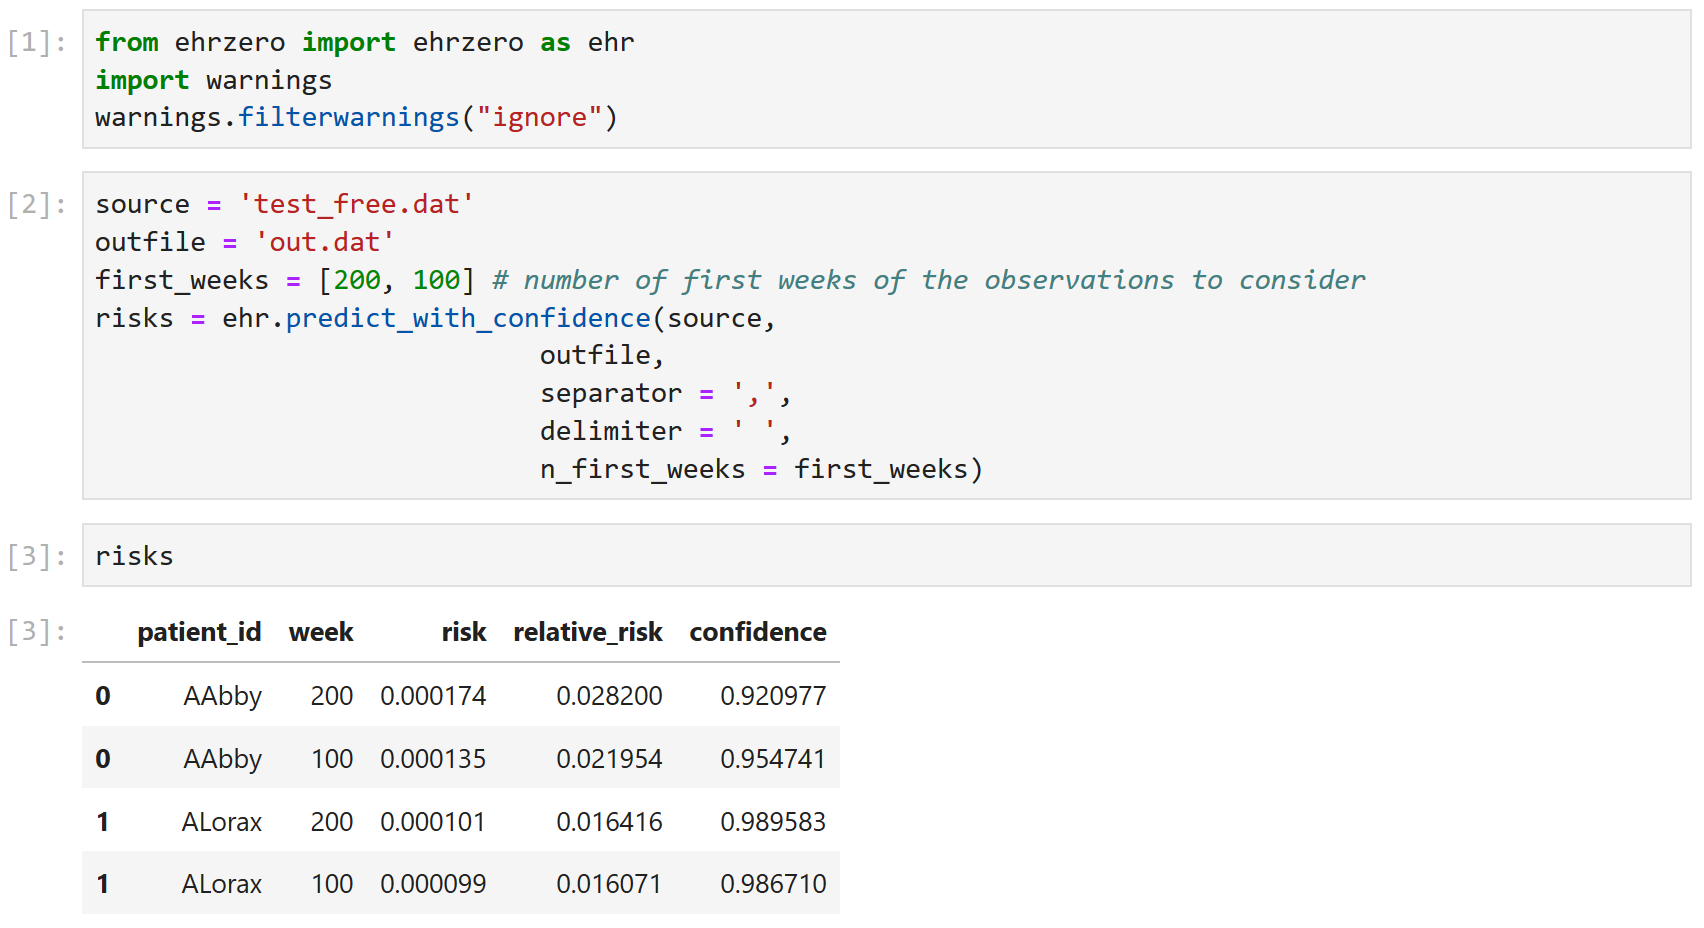
\includegraphics[width=.9\textwidth]{Figures/ehrzero_example}
\captionN{Python code prediction example}
\end{figure}

%###################################
\subsection{Prerequisites \& Installation}

The minimum prerequisites for running ehrzero are the following:
\begin{enumerate}
\item A x64 system running any flavor of Linux.
\item A working python 3.x installation
\item \texttt{scikit-learn}, version = \texttt{0.20.0}
\end{enumerate}

Installation:

\texttt{pip3 install ehrzero --user}

\subsection{EHR data format}

Diagnostic data stored in text file, one line per patient as follows: patient id, gender, and list of space-separated, comma-delineated diagnosis records, all separated by spaces. Each diagnosis record consists of the week since the start of the  observation, followed by a comma,  and the ICD-9 code of the diagnosis. 

Example of a patient line:

\texttt{Lorax,M 5,277.03 10,611.79 18,057.8 58,157.8 78,057.8 108,057.8 128,057.8 148,057.8}

\subsection{Sample Python code risk estimation}

Once the patient diagnostic data is in the required format, for function \texttt{predict\_with\_confidence} we specify the filepath of the data and the list of the cutoffs for the first weeks since the start of observations for the data we want to analyze. We also specify the separator and delimiter for the patients within file (space and comma are default values, but can be changed for user convenience).

The \texttt{predict\_with\_confidence} function returns the predicted risk of autism for every patient in the input file with all the specified numbers of first weeks to consider.

\subsection{Sample Python script risk estimation}

The script version is similar to the one mentioned before.

Once \texttt{ehrzero} package is installed, locate its directory and go to texttt{../ehrzero/example}. Select one of the \texttt{".dx"} or \texttt{".dat"} files in \texttt{/ehrzero/example/tests} as input and run the following command as an example:

\texttt{python zero.py -data tests/ZERO$\-$example.dat -outfile predictions.csv -n$\-$weeks 100 200 300 -Verbose 1}

\begin{figure}[!ht]
\centering
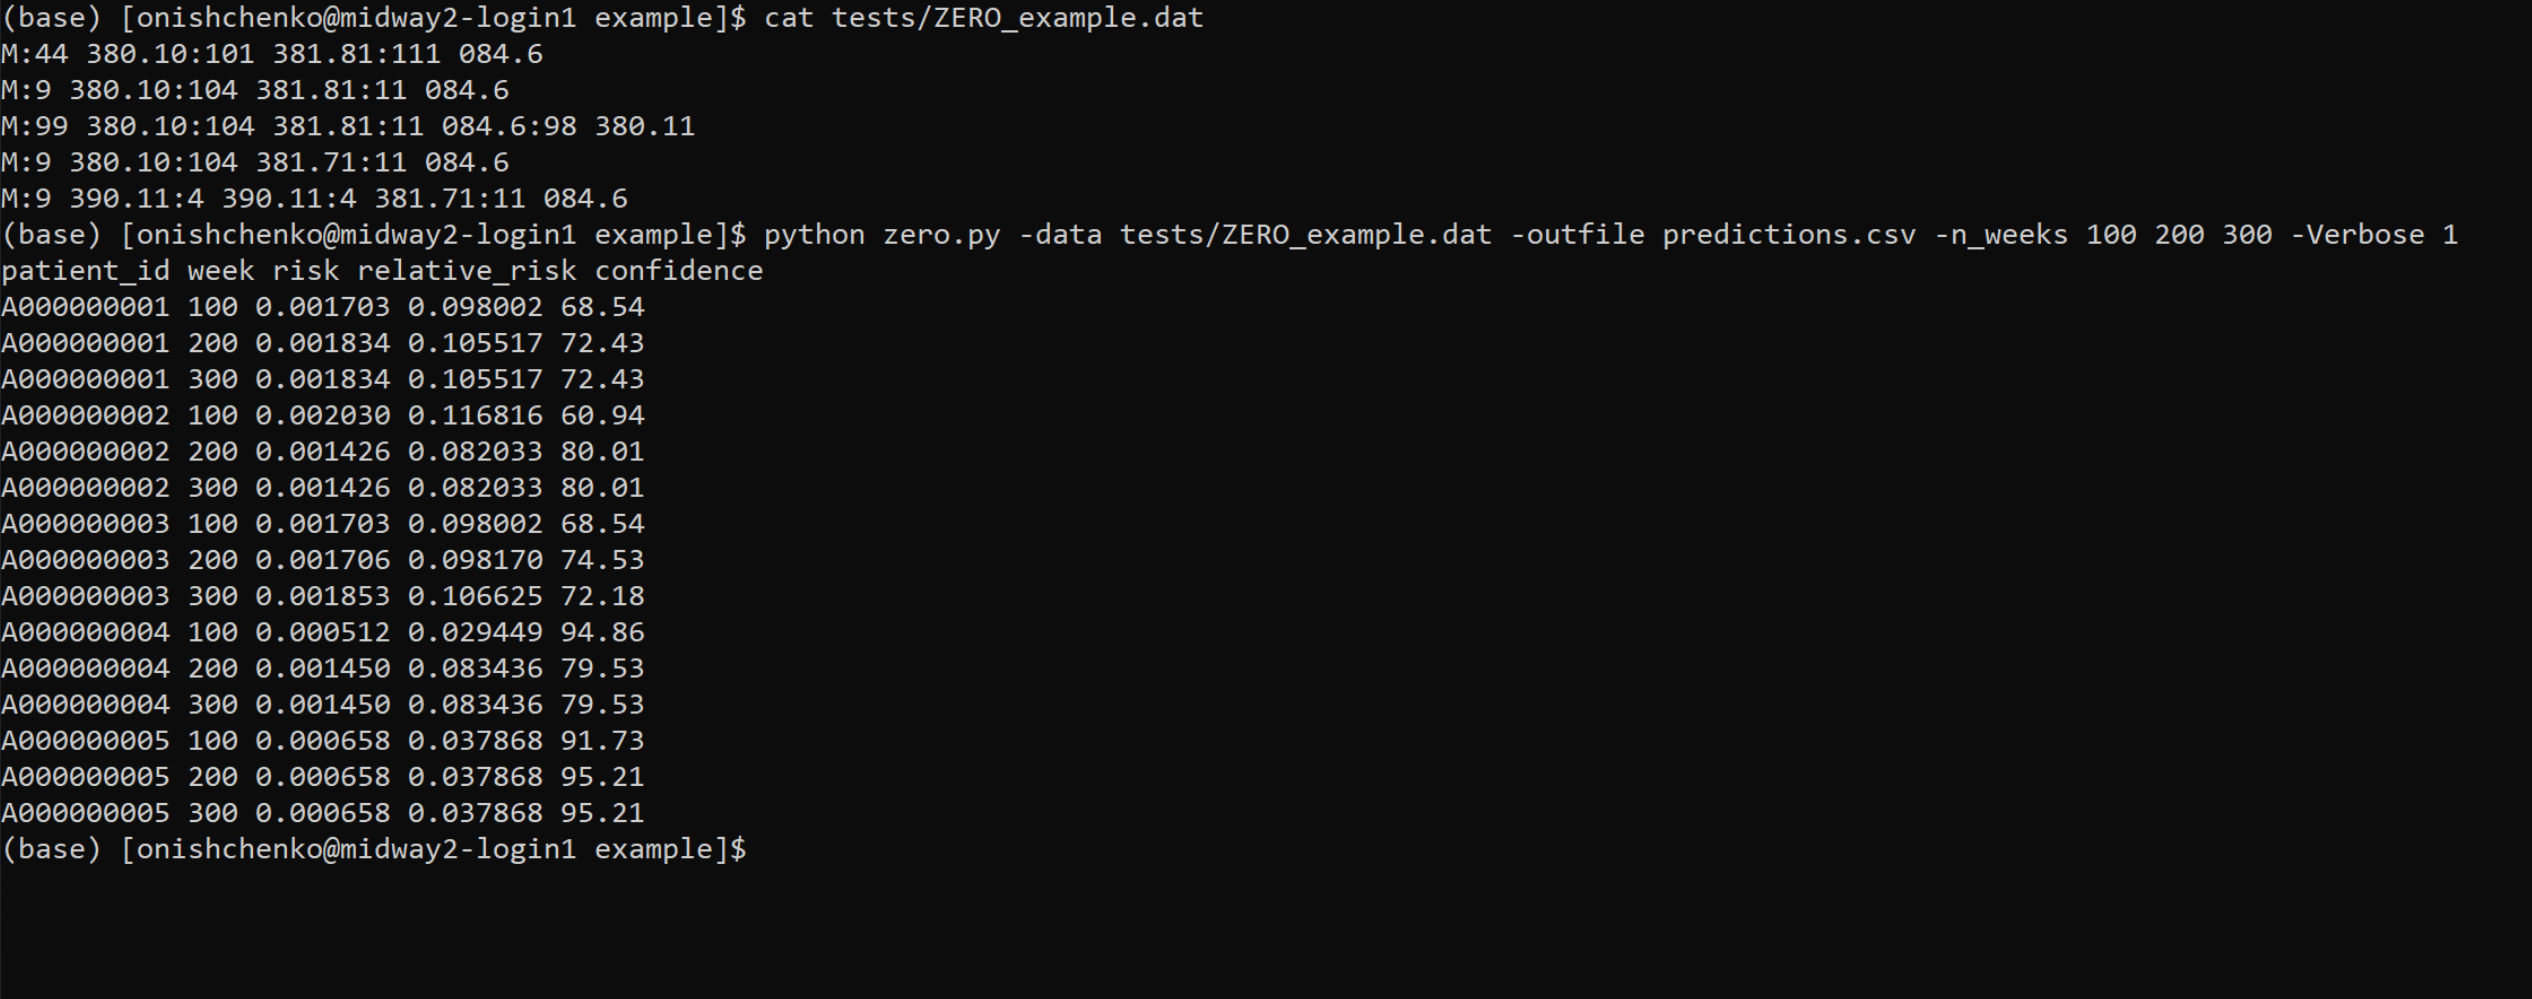
\includegraphics[width=.9\textwidth]{Figures/zero_py_example}
\captionN{Python script prediction example}
\end{figure}